\documentclass[12pt]{article}
\usepackage[a4paper,bindingoffset=0.2in,left=2.5cm,right=2.5cm,top=1.5cm,bottom=1.5cm,footskip=.25in]{geometry}
\usepackage{graphicx}
\usepackage{caption}
\usepackage{subcaption}
\usepackage{placeins}
\usepackage{amsmath}
\usepackage{hyperref}
\usepackage[export]{adjustbox}

%================================
\title{Analysis of Drift in Knee Joint Angle}
\author{Sandeep Kumar}


\begin{document}
\maketitle


\section*{Problem}

We are using two IMU sensors, one mounted on thigh and the shank to calculate the Knee joint angle (Flexion and Extension).\\
We are using the techniques mentioned in the paper \cite{s140406891} and \cite{conf/IEEEcca/SeelSR12} to do so.\\

One of the method mentioned in the papers uses only Gyroscope data to calculate the Joint Knee angle.\\

Result of using that algorithm on the data gather from the EXL IMU sensors is shown in the Figure \ref{exlgyrosangle}

\begin{figure}[!htb]
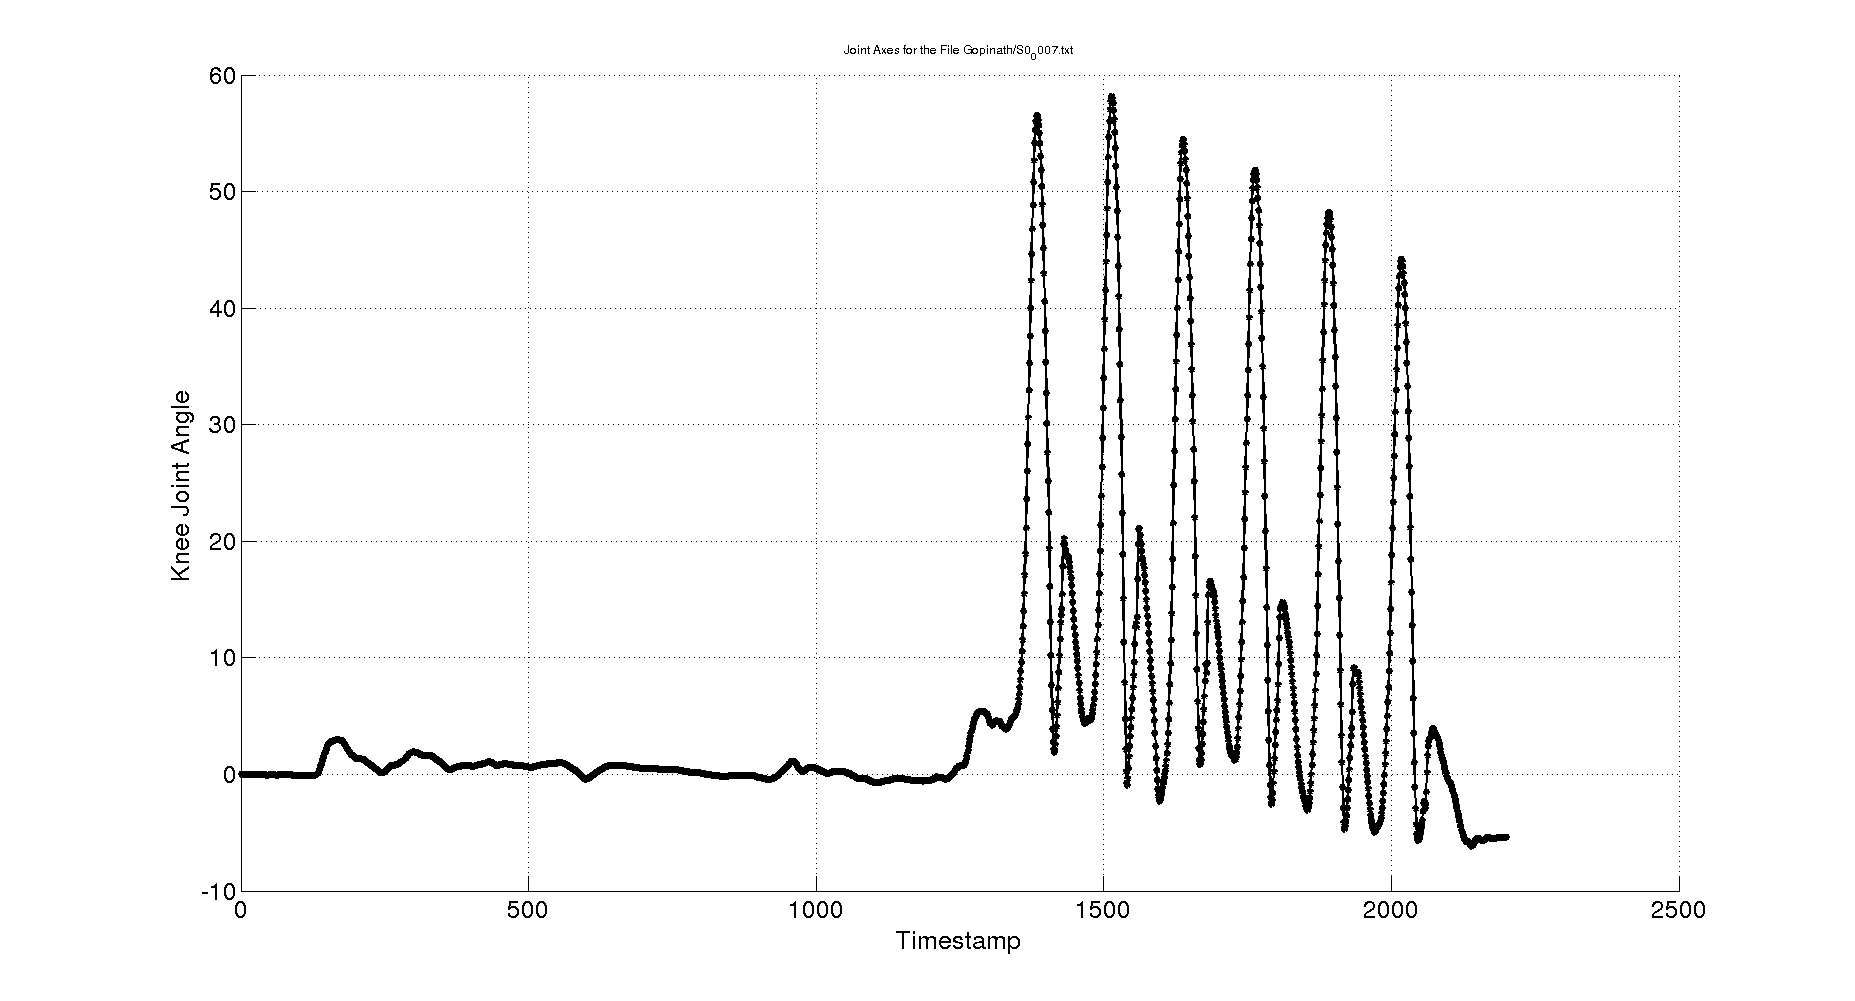
\includegraphics[scale=.32,left]{problem.png}
\caption{Knee Joint Angle Calculated using only Gyroscope Data\\
\scriptsize{Data generation was started before the subject starts walking, and hence the long flat line in the beginning }
}
\label{exlgyrosangle}
\end{figure}

The problem we are facing is that the Knee Joint angle, keeps going down with each of the step, as shown in the Figure \ref{exlgyrosangle}. We need to figure out whether this is because of the method we are using, or there is a problem in the data sent by the Gyroscope to us.

\section*{Brief Overview on how it is calculated}

According to the methods mentioned in the \cite{s140406891} and \cite{conf/IEEEcca/SeelSR12} we can mount the sensors on the thigh and the shank with any orientation. There is no requirement that on of the principal axis of the sensor must coincide with that of the joint center axis, as shown in the Figure \ref{kneeinfo}.\\
The first part in the calculation of the Knee joint angle is to figure out the Knee Joint center Axis and Knee Joint center coordinate with respect to local coordinate system of both of the sensors. There will be $ j_1 $ and $ j_2 $ Knee joint center axes with respect to sensor 1 and sensor 2 (the blue line, line from sensors to the center of the knee joint) and similarly $ o_1 $ and $ o_2 $ , the Knee Joint center coordinate with respect to sensor 1 ad sensor 2.\\


\begin{figure}[!htb]
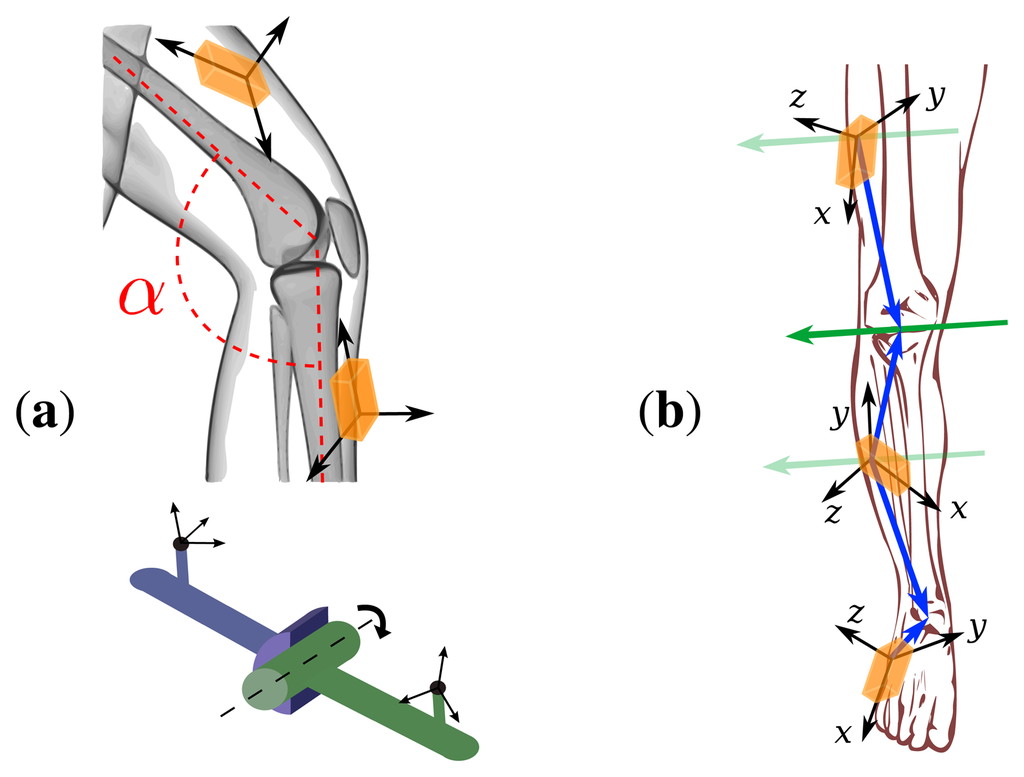
\includegraphics[scale=2,center]{jointAxis.png}
\caption{Figure showing the Joint Knee angle, and the Knee Joint Center Axes}
\label{kneeinfo}
\end{figure}

\subsection*{Using only Gyroscope Data}
We just need $ j_1 $ and  $ j_2 $ to calculate knee joint angle using only  Gyroscope data. Joint center coordinates are required during the calculation of the angle using Accelerometer data.\\

Joint center axis $ j_1 $ and $ j_2 $ can be calculated using the kinematic constraints in a Hinge Joint. $ g_1(t) $ and $ g_2(t) $ (The angular velocity as noted by the Gyroscope in the two sensors respectively.) differ only by the joint angle velocity and a time variant rotation matrix. Hence their projections into the joint plane(the plane to which the joint axes is the normal vector) have the same lengths for each instant in time.


\begin{equation}\label{eq:projectZero}
{\lVert}g_1(t) \times j_1 {\rVert}_2 - {\lVert}g_2(t) \times j_2 {\rVert}_2 = 0\text{ } \forall t
\end{equation}
where $ \lVert . \rVert _2 $ dentoes the Euclidean norm. \vspace{1em}

\textbf{Basically it says that if we project the angular velocity of the sensors, into the Joint plane (Place to which Joint center axis is normal), there length should be same.}\\

We have $ g_1(t) $ and $ g_2(t) $, we need to find $ j_1 $ and $ j_2 $. For this we randomly assign some value to $ j_1 $ and $ j_2 $  and using Gauss-Newton algorithm or any other standard optimization method.

The calibration data is used for this. After the optimization part \ref{eq:projectZero} should hold (approximately). Figure \ref{diffproject} shows the difference.

\begin{figure}[!htb]
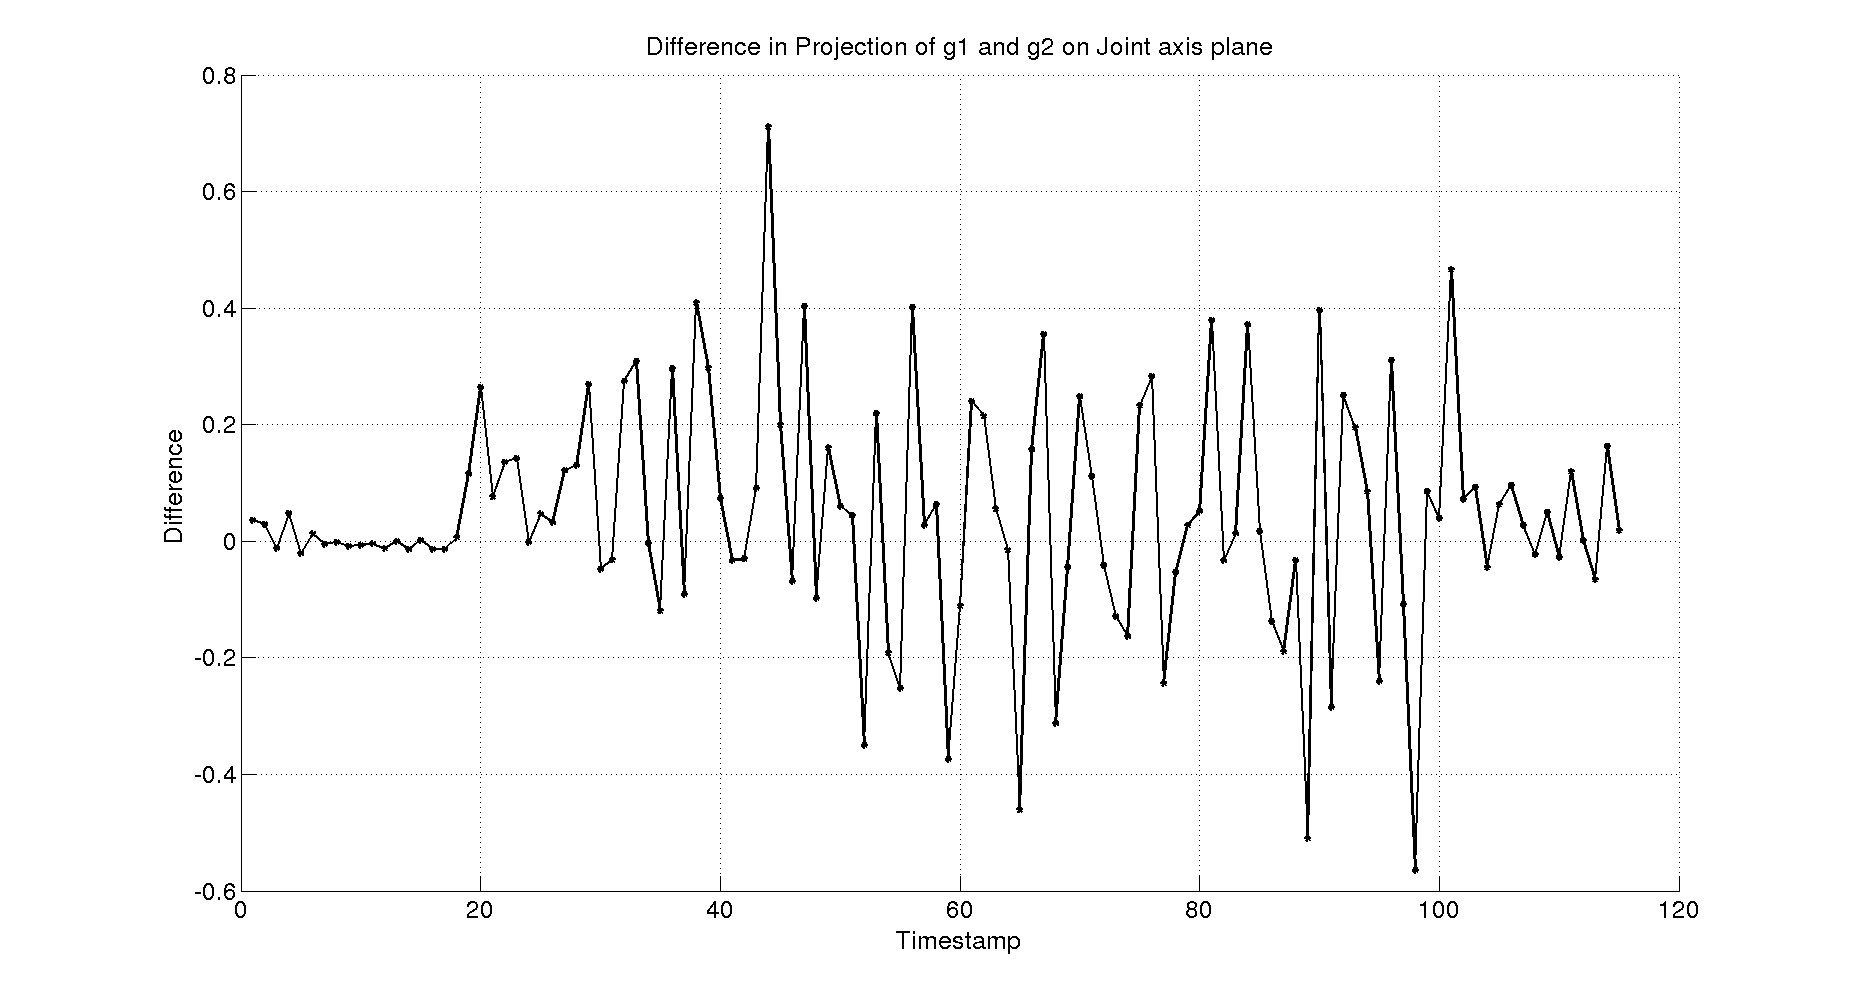
\includegraphics[scale=.3,center]{diffproject.png}
\caption{Difference in the projection of g1 and g2 on j1 and j2 respec.}
\label{diffproject}
\end{figure}
\FloatBarrier
We can see in the Figure \ref{diffproject} see that the difference is close to zero (it can be argued that if it  is possible to improve it further), we can assume that the calibration part is working correctly, and any drift appearing in the final result does not come from here.\\

\textit{There was a concern that the difference here is show in radians and need to be converted to degrees for the final evaluation. However that is not correct as the graph shows the difference, as shown in the equation \ref{eq:projectZero}. So converting the difference to degrees is not correct.}\\

After obtaining Joint center axis, a gyroscope-based flexion/extension angle can be calculated by integrating the difference of the angular rates around the respective joint axis, i.e.

\begin{equation}
\alpha_{gyr}(t) = \int_0^t(g_1(\tau).j_1 - g_2(\tau).j_2)d\tau
\end{equation}

In Matlab this can be coded as:\\

\begin{verbatim}
for i=2:size(gyro_s_knee,2)
    proj1(i-1) = dor(gyro_s_knee(:,i-1), j1_valf) ;
    proj2(i-1) = dot(gyro_s_shank(:,i-1), j2_valf);
    dproj1(i-1) = radtodeg(dot(gyro_s_knee(:,i-1), j1_valf));
    dproj2(i-1) = radtodeg(dot(gyro_s_shank(:,i-1), j2_valf));
    
    angle_joint_axes (i) = angle_joint_axes (i-1) +...
        radtodeg((proj2(i-1) - proj1(i-1)) * t);
end
\end{verbatim}




\newpage
\section*{Problem in Data or Algorithm}

The Knee joint angle that we are currently getting using only Gyroscope data, looks like this.
\begin{figure}[!htb]
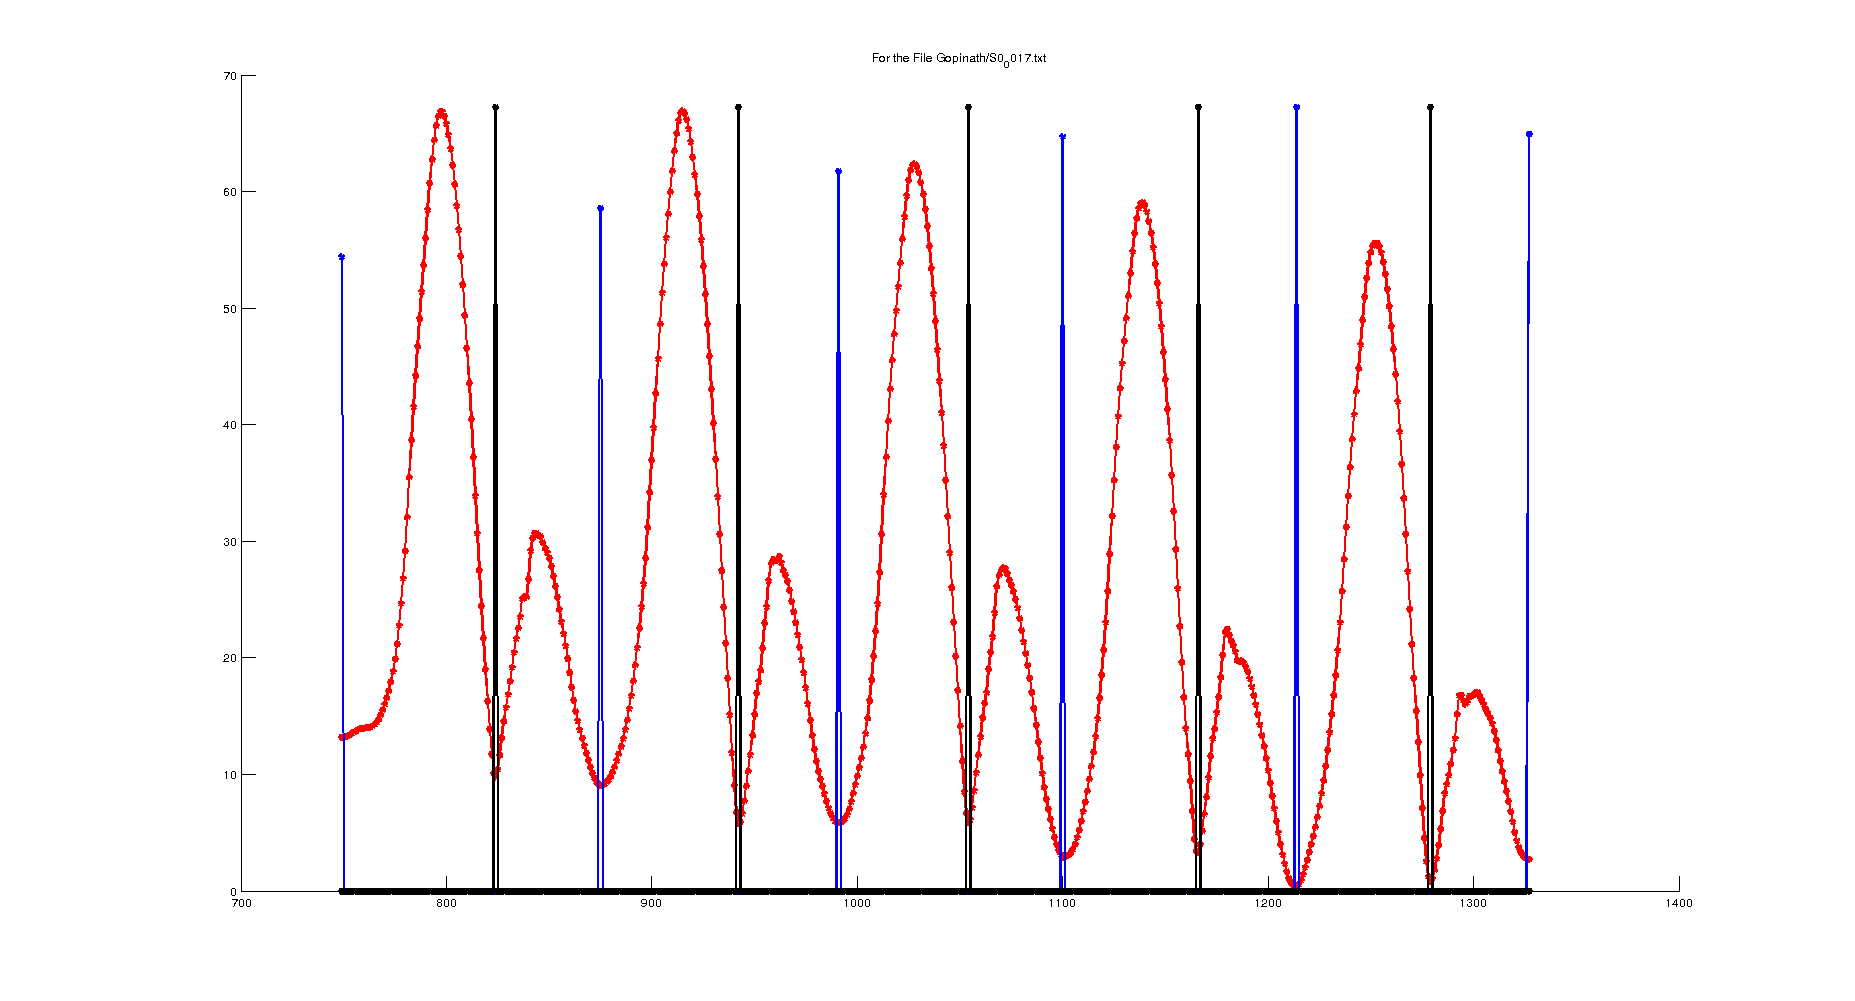
\includegraphics[scale=.3,center]{driftSteps.png}
\caption{Walk as captured by the EXML IMU Sensors using Gyro Data. Drift is present here.}
\label{diffproject}
\end{figure}

We can clearly that there is a drift in the angles, (it goes down with each step in the walk). As mentioned in \cite{s140406891},\textit{\textbf{ the gyroscope-based angle is very precise on short time scales, but exhibits some slow drift of about 1.5 degree/sec. The drift depends on the bias of the gyroscope.
}}\\

When we manually correct the drift by adding the loss of the angles over the period of time, the walk looks like this:
\begin{figure}[!htb]
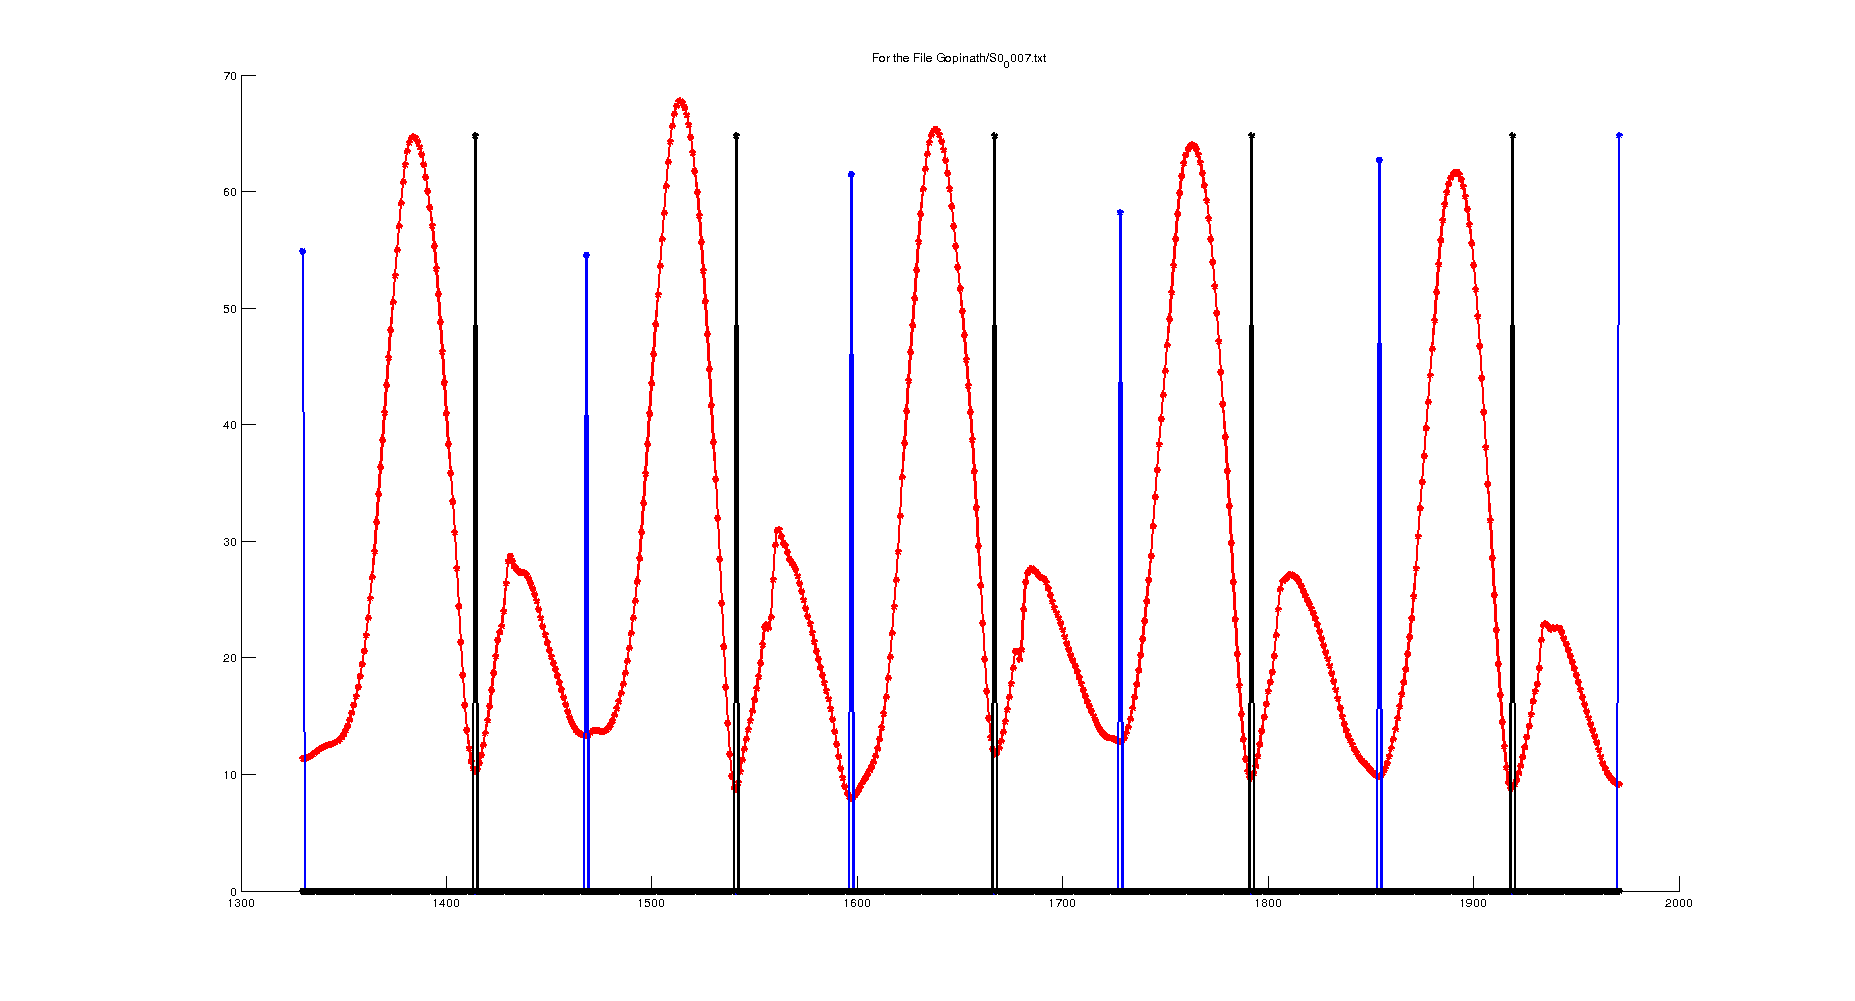
\includegraphics[scale=.3,center]{driftFreeSteps.png}
\caption{Walk as captured by the EXML IMU Sensors using Gyro Data. Drift free walk.}
\label{diffproject}
\end{figure}

As we can clearly see that the walk is free from the drift. From this we can infer that the drift present is due to Gyroscope and not because of the algorithms used. We present some possible solutions to fix this in the next section.
\FloatBarrier

\section*{Possible Solutions}

Even though the paper says that the Knee angle calculated using only the Gyroscope values will be close to the actual value, they accept that sometimes the results can be affected by drift.\\

\begin{quote}
\textit{The hinge joint angle can be calculated by integrating the difference of both angular rates around the corresponding coordinate axis. Since even the most precise calibration will yield a non-zero bias, this calculated angle will be subject to drift.}
\end{quote}

The solution is to combine the Gyroscope angle, with a noisy, but drift less, joint angle estimate that is calculated from the measured accelerations.\\

Here is the angle calculated by only using the Accelerometer data.\\
\begin{figure}[!htb]
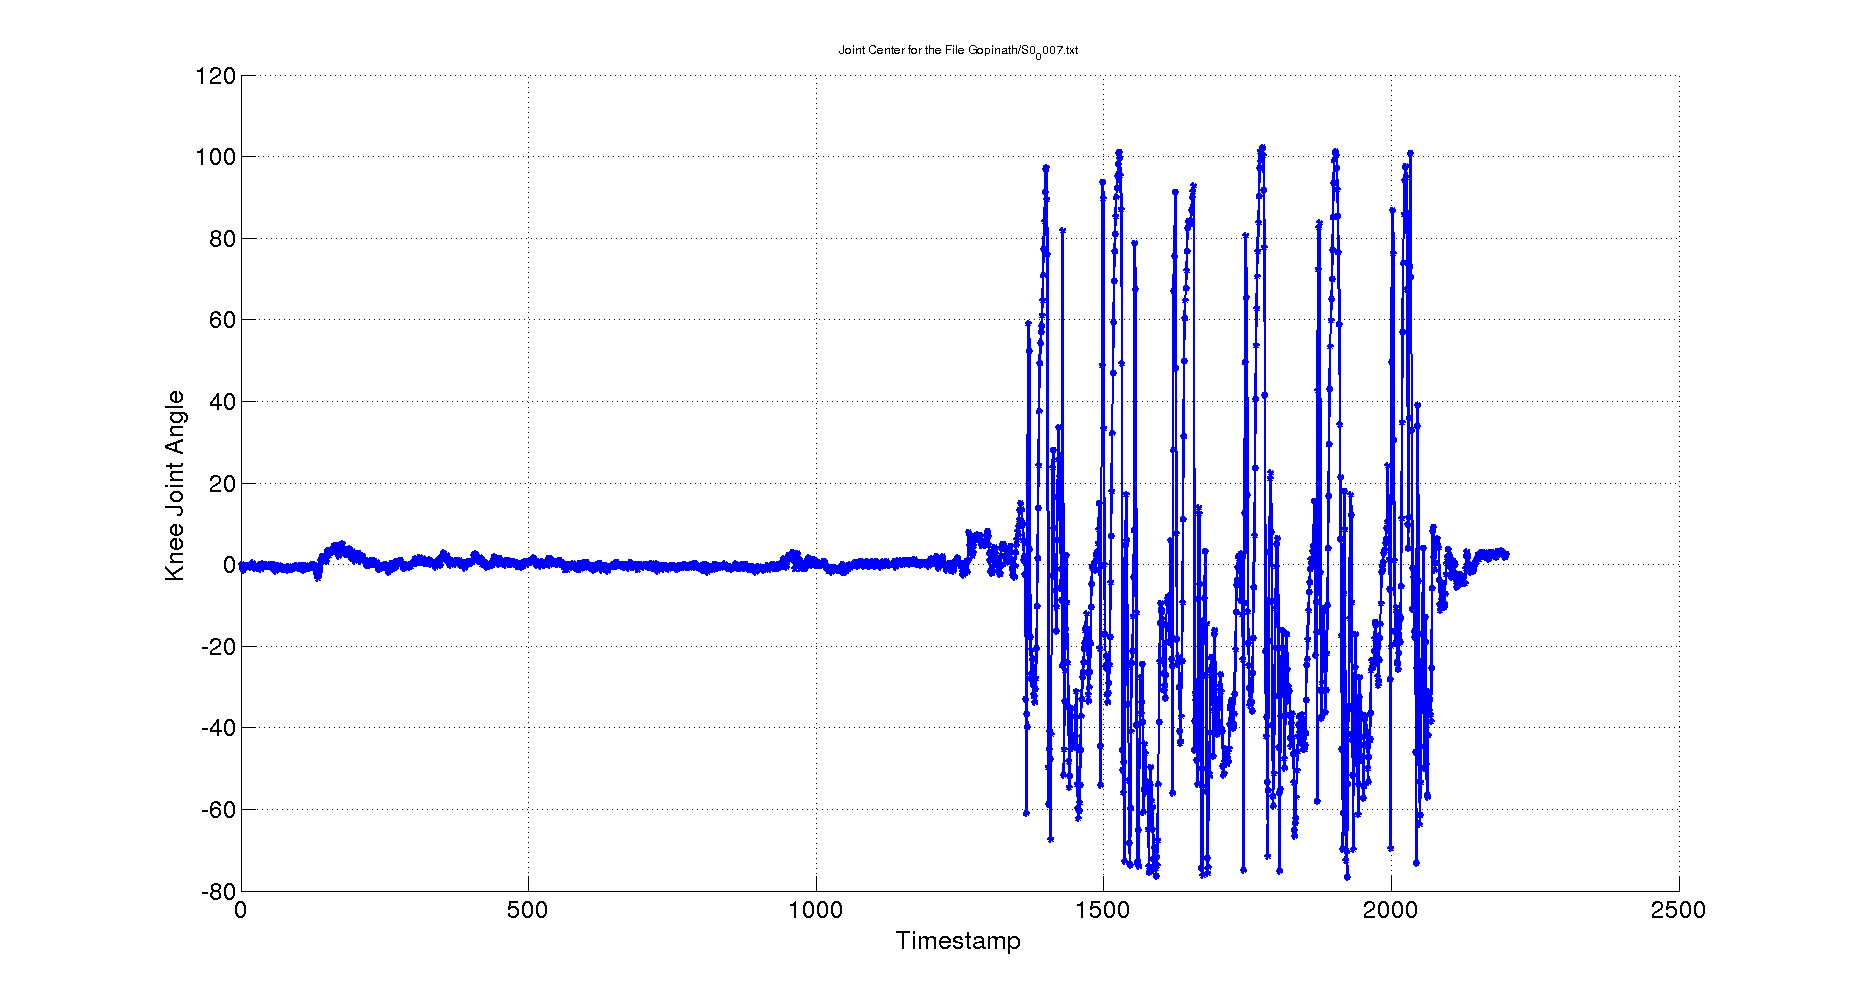
\includegraphics[scale=.3,center]{noisyacceangle.png}
\caption{Noisy but drift less Knee Joint Angle using Accelerometer. Range of the angles is also higher than that the angle obtained by using the Gyroscope data.}
\label{diffproject}
\end{figure}

\FloatBarrier

We can see that, though the data is noisy there is no drift in it. We can combine the two angles using a complementary filter or a Kalman filter.\\
Angles can be combined using equation \ref{accplusgyro}
\begin{equation}\label{accplusgyro}
\alpha_{acc+gyr}(t) = \lambda \alpha_{acc}(t) +(1-\lambda)(\alpha_{acc+gyr}(t-\Delta t)+\alpha_{gyr}(t) - \alpha_{gyr}(t-\Delta t)), \vspace{2em} \lambda \in [0,1]
\end{equation}
In Matlab this can be implemented like:

\begin{verbatim}
lambda = 0.01;
deltaT = 2; % 0.02 sec
angle_FE3(1,1) = angle_joint_axes(1,1);
angle_FE3(1,2) = angle_joint_axes(1,2);

for t = 3:data_size
    angle_FE3(1,t) = lambda*angle_joint_centre(1,t) +(1-lambda)*...
    (angle_FE3(1,t-deltaT)+angle_joint_axes(1,t)-angle_joint_axes(1,t-deltaT));
end
\end{verbatim}

Here is a plot of the combined angle looks like:
\begin{figure}[!htb]
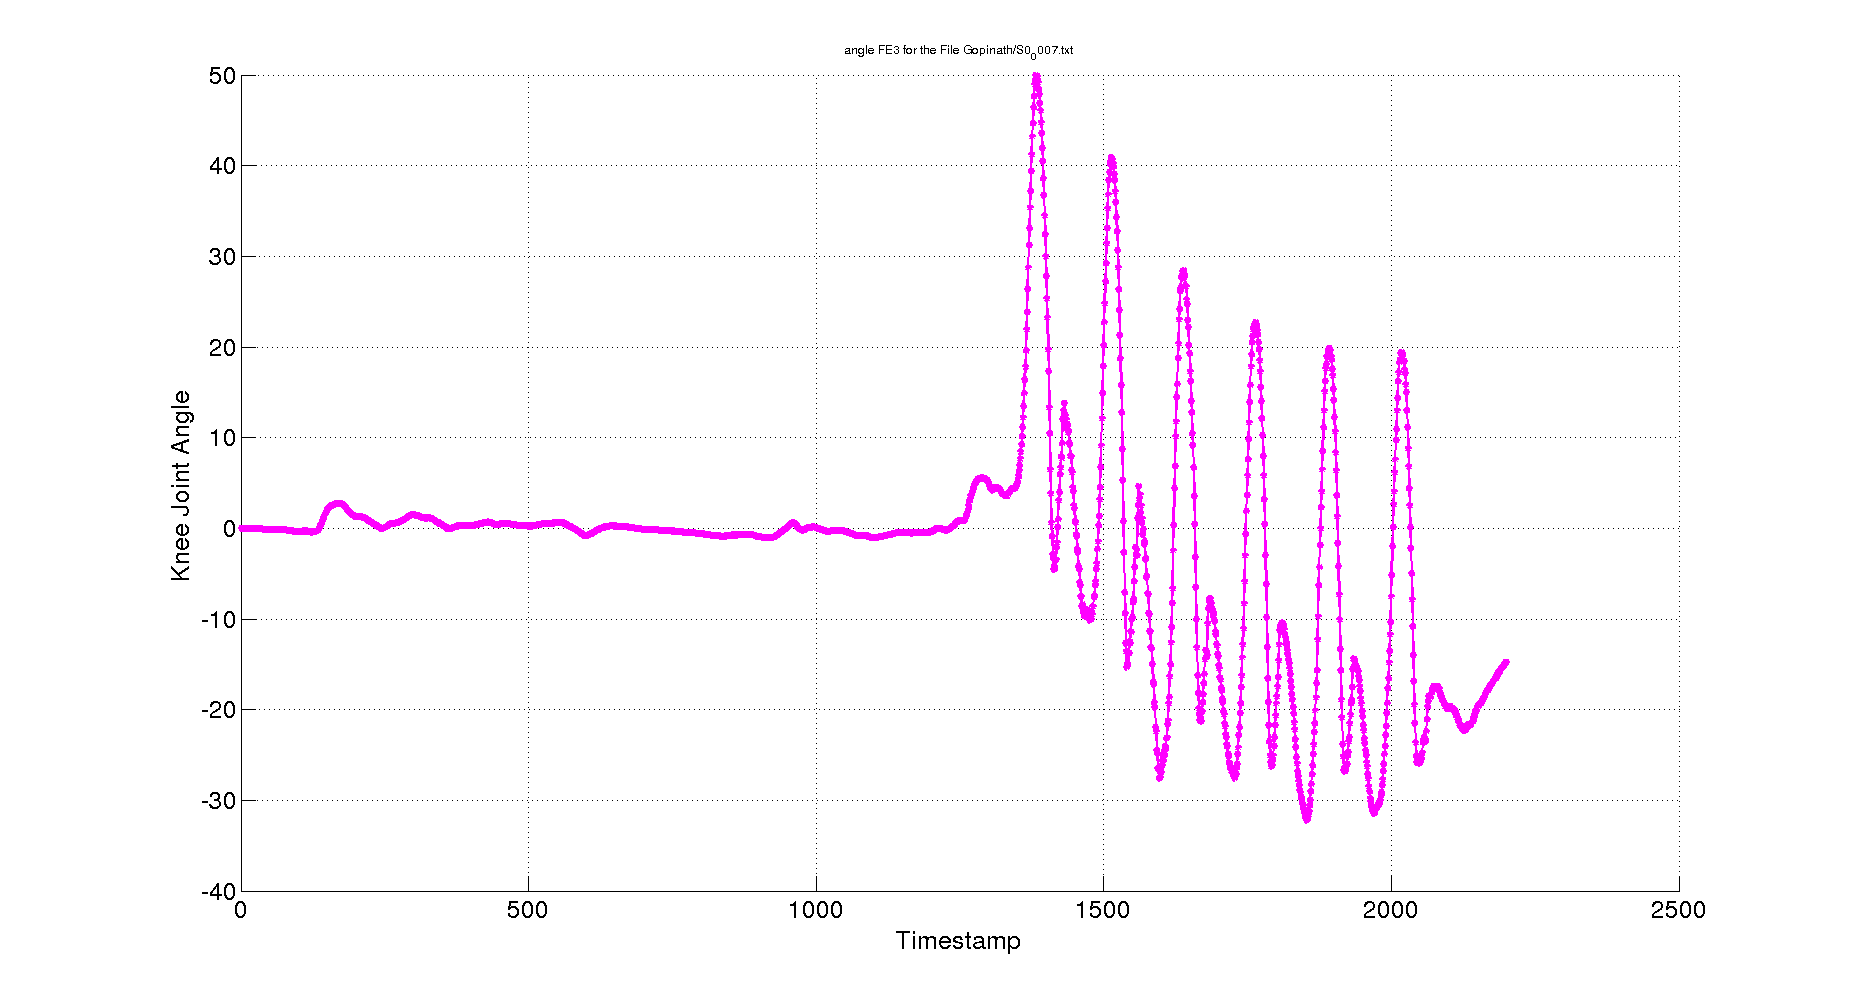
\includegraphics[scale=.3,center]{accplusgyro.png}
\caption{Combined Knee Joint Angle using $ \lambda = 0.01 $ and $ \Delta t = 0.02 $ sec}
\label{diffproject}
\end{figure}

The value of the hyper-parameters $ \lambda $ and $ \Delta t $ controls the final Flexion Extension angle. We need to find the proper values of these hyper-parameters to get the desired result.

Please note that the the angle obtained by the using accelerometer in the paper \cite{s140406891} is less noisy, as can be seen in the Figure \ref{lessDrifrinPaper}

\begin{figure}[!htb]
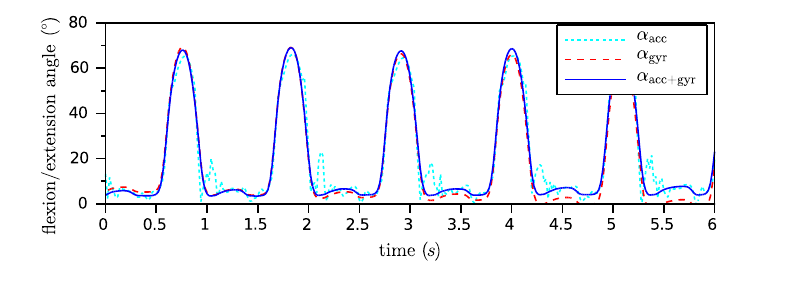
\includegraphics[scale=.6,center]{lessDriftinPaper.png}
\caption{Knee Joint angle as obtained using, Gyrometer, Accelerometer, and a combination of both of them using the equation \ref{accplusgyro} and values of the hyper-parameters as $ \lambda = 0.01 $ and $ \Delta t = 0.02 $ sec}
\label{lessDrifrinPaper}
\end{figure}
\FloatBarrier

The noise which they are getting is very low when compared to the noise that we are getting in angles obtained from using accelerometer. We need to see that whether \ref{accplusgyro} is the correct way to proceed further or we need some other method for this  purpose.

\bibliography{mybib}{}
\bibliographystyle{plain}
\end{document}